\documentclass[addpoints]{exam}
\input{../preamble}

\firstpageheader{AP Physics}{Chapter 6 Problem Set 1}{Name:\enspace\makebox[1.25in]{\hrulefill}}

\CorrectChoiceEmphasis{\color{red}\bfseries}
\SolutionEmphasis{\color{red}}
\begin{document}

\begin{center} \fbox{\fbox{\parbox{5.5in}{\textbf{Directions}: Please view the back side of this paper to view instructions and advice.

\begin{center}
    \textbf{EQUATIONS}
\end{center}
\vspace{-1em}

\begin{equation*} 
    F = \frac{G m M}{r^2} \hspace{2em}
    G = \SI{6.674e-11}{\frac{N \cdot m^2}{kg^2}} \hspace{2em}
    g = \frac{G M}{r^2}
\end{equation*}
}}}
\end{center}

\begin{questions}
\printanswers

\question
The distance between two spheres of mass \SI{850}{kg} and \SI{970}{kg} is \SI{2.00}{m}. What is the gravitational force between the spheres?

\begin{solution}

\begin{equation*}
    F = \frac{G m M}{r^2} = \SI{1.38e-5}{N}
\end{equation*}
\end{solution}

\question 
What is the distance between the centers of mass for the objects below?
\vspace{-2em}

\begin{figure}[h!]
    \centering
    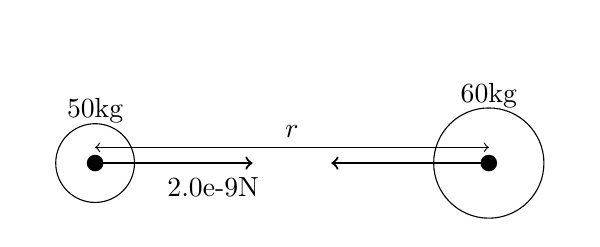
\begin{tikzpicture}
        \fill (0,0) circle[radius=3pt]; %node[below] {\tiny CM};
        \fill (5,0) circle[radius=3pt]; %node[below] {\tiny CM};
        \draw[<->] (0,0.2) -- (5,0.2);
        \node at (2.5,0.4) {$r$};
        \draw (0,0) circle (0.5cm) node[above,inner sep=0.5cm] {\SI{50}{kg}};
        \draw (5,0) circle (0.7cm) node[above,inner sep=0.7cm] {\SI{60}{kg}};
        \draw[->,thick] (0,0) -- (2,0);
        \draw[->,thick] (5,0) -- (3,0) ;
        \node at (1.5,-0.3) {\SI{2.0e-9}{N}};
        % \node at (3.8,-0.25) {$F$};
    \end{tikzpicture}
\end{figure}

\begin{solution}
Solving Newton's law of universal gravitation for distance leads to

\begin{equation*}
    r = \sqrt{\frac{GmM}{F}} = 
    \sqrt{\frac{\left(\SI{6.674e-11}{\frac{N \cdot m^2}{kg^2}}\right) \left(\SI{50}{kg}\right) \left(\SI{60}{kg}\right)}{\SI{2.0e-9}{N}}} = \SI{10.0}{m}
\end{equation*}
\end{solution}

\question 
The acceleration due to gravity on planetary bodies may be calculated using knowledge of mass and radius. For the parts below, use Eq.~(6.43) in your calculations and reference the NASA Planetary Fact Sheet (\href{https://nssdc.gsfc.nasa.gov/planetary/factsheet/}{link}).

\begin{parts}
\part What is the acceleration due to gravity on Earth?

\part What is the acceleration due to gravity on the Moon?

\begin{solution}

\begin{equation*}
    g = \frac{G M}{r^2} = \frac{(\SI{6.674e-11}{\frac{N \cdot m^2}{kg^2}})(\SI{7.3e22}{kg})}{(\SI{1.738e6}{m})^2} = \SI{1.6}{m/s^2}
\end{equation*}
\end{solution}

\part What is the acceleration due to gravity on Mars?

\begin{solution}

\begin{equation*}
    g = \frac{G M}{r^2} = \frac{(\SI{6.674e-11}{\frac{N \cdot m^2}{kg^2}})(\SI{6.42e23}{kg})}{(\SI{3.396e6}{m})^2} = \SI{3.71}{m/s^2} 
\end{equation*}
\end{solution}

% \part What is the acceleration due to gravity on the Sun?

\begin{solution}

\begin{equation*}
    g = \frac{G M}{r^2} = \frac{(\SI{6.674e-11}{\frac{N \cdot m^2}{kg^2}})(\SI{1.99e30}{kg})}{(\SI{6.96e8}{m})^2} = \SI{274}{m/s^2} 
\end{equation*}
\end{solution}
\end{parts}

\question
By what factor does the gravitational force between two objects change when the distance between them increases by a factor of 13?

\begin{solution}

\begin{equation*}
    \frac{F_{\text{new}}}{F_{\text{old}}} \sim \frac{G m M}{r^2} = \frac{(1)(1)(1)}{(13)^2} = \SI{5.9e-3}{} 
\end{equation*}
\end{solution}

\question
By what factor does the gravitational force between two objects change when the objects are brought $6 \times$ closer?

\begin{solution}

\begin{equation*}
    \frac{F_{\text{new}}}{F_{\text{old}}} \sim \frac{G m M}{r^2} = \frac{(1)(1)(1)}{\left(\frac{1}{6}\right)^2} = 6^2 = 36
\end{equation*}

The gravitational force gets 36 times stronger.
\end{solution}

\question
Let $F$ be the gravitational force between Earth and the Moon. If Earth was $10 \times$ more massive, the Moon was $4 \times$ more massive, and the distance between the bodies was $5 \times$ greater, by what factor would $F$ change? Does $F$ increase or decrease? 

\begin{solution}

\begin{equation*}
    \frac{F_{\text{new}}}{F} \sim \frac{G m M}{r^2} = \frac{(1)(10)(4)}{(5)^2} = \frac{40}{25} = 1.6
\end{equation*}

The gravitational force would increase by a factor of 1.6.
\end{solution}

\question
Consider a \SI{9.25}{lbs} baby sleeping in a crib. 

(Note: $\SI{1}{kg} = \SI{2.205}{lbs}$)

\begin{parts}
\part Calculate the gravitational force on the baby by the baby's \SI{135}{lbs} father, who stands \SI{30}{cm} away. 

\begin{solution} 
The separation distance is $r = \SI{30}{cm} = \SI{0.30}{m}$.
The masses of the baby and father are

\begin{equation*}
    m = \SI{9.25}{lbs} \times \frac{\SI{1}{kg}}{\SI{2.205}{lbs}} = \SI{4.20}{kg}
\end{equation*}
\vspace{-1em}

\begin{equation*}
    M = \SI{135}{lbs} \times \frac{\SI{1}{kg}}{\SI{2.205}{lbs}} = \SI{61.2}{kg}
\end{equation*}

\begin{equation*}
    F = \frac{G m M}{r^2} = \SI{1.9e-7}{N}
\end{equation*}
\end{solution}

\part Calculate the gravitational force on the baby by Jupiter, which is 390 million miles away.  

(Note: $\SI{1}{mi} \approx \SI{1609}{m}$)

\begin{solution} 
By the \textit{Planetary Fact Sheet} Jupiter's mass is $M = \SI{1.898e27}{kg}$. The distance between Jupiter and the baby is

\begin{equation*}
    r = \SI{390e6}{mi} \times \frac{\SI{1609}{m}}{\SI{1}{mi}} = \SI{6.28e11}{m}
\end{equation*}

The gravitational force by Jupiter is

\begin{equation*}
    F = \frac{G m M}{r^2} = \SI{1.3e-6}{N}
\end{equation*}
\end{solution}

% \part
% Calculate the gravitational force on the baby by the Sun.

% \begin{solution} 
% $M = \SI{1.989e30}{kg}$. The distance between the Earth and Sun is $r = \SI{1.496e11}{m}$.

% The gravitational force by the Sun is

% \begin{equation*}
%     F = \frac{G m M}{r^2} = \SI{2.49e-2}{N}
% \end{equation*}
% \end{solution}

% \part 
% Calculate the gravitational force on the baby by Earth. How does this force compare to the baby's weight, $w$?

% \begin{solution} 
% $M = \SI{5.9736e24}{kg}$, $r = R_{\mathrm{\Earth}} = \SI{6.376e6}{m}$.

% The gravitational force by Earth is

% \begin{equation*}
%     F = \frac{G m M}{r^2} = \SI{41.2}{N}
% \end{equation*}

% This force is exactly equal to the baby's weight, $w = mg$.
% \end{solution}

% \part
% Rank order the gravitational forces in the previous parts from least to greatest magnitude.


\part 
Compare the gravitational force from the father with the force from Jupiter. (Take their ratio.)

\begin{solution}
Jupiter exerts a gravitational force on the baby that is $7 \times$ greater than the force from the father.
\end{solution}
\end{parts}

\clearpage

\textbf{Instructions and Advice}
\begin{enumerate}
\setlength\itemsep{0.1ex}
    \item Show your work and answers on separate sheets of paper. Staple those sheets to this one. Although you don't need to staple extra scratch paper that you used for side calculations or brainstorming, your final product should be a detailed and organized solution of the problems.
    \item Start early. You'll probably have questions. Some problems are similar to those we cover in class. Review your class notes as you work on these problems.
    \item When in doubt, employ the GUESS method: Write the known quantities, the unknown, and equation(s) relating the known and unknown. Solve equations for the unknown. Substitute numbers at the \textit{end} of a problem.
    \item Use Desmos (available at \href{https://www.desmos.com/scientific}{https://www.desmos.com/scientific}).
    \item Don't give up on a problem without trying your best. Ask Mr.~Nunez and your peers for help.
    \item Keep in mind that future quizzes and tests are based in part on these problem sets. You should use these practice problems as a study guide.
    \item Write solutions that will make sense to \textit{you} one week from today.
    \item Practice makes you better. Re-visit these problems even after you solve them. Solving problems without looking at your notes will refine your problem-solving skills.
\end{enumerate}


\end{questions}
\end{document}